\documentclass[titlepage]{article}
%\usepackage[T1]{fontenc}
%\usepackage[utf8]{inputenc}
%\usepackage{lmodern}
%\usepackage{babel}
\usepackage{amssymb}
\usepackage{amsmath}
\usepackage[table]{xcolor}
\usepackage{booktabs}
\usepackage[hidelinks]{hyperref}
\usepackage{tabularx}
\usepackage{graphicx}
\usepackage{acronym}
\usepackage{float}
\usepackage[font=normal, labelfont = bf]{caption}
\usepackage{sidecap}
\usepackage{rotating}
\usepackage{rotfloat}
\usepackage[ampersand]{easylist}
\usepackage{multirow}

%%% page parameters
\oddsidemargin 1 cm
\textwidth 14cm
\topmargin -1 cm
\textheight 23 cm

\setcounter{tocdepth}{2}
\title{Robot User Manual}
\author{Group 2   {\em Coding Pharaohs}\\ 
\\
Abdulaziz ALHULAYFI a1642362  \\
Yu HONG	 a1616861  \\
Jianqiu LI a1635717  \\
Matthew NESTOR a1132338  \\
Yifei PEI a1611648  \\
Bowen TAO a1622211}  
\date{\today}
\begin{document}
\maketitle
\tableofcontents

\pagebreak

\pagebreak



\pagebreak

%%INTRODUCTION
\section{Introduction}
This document provides guidence for the operator on how to use the robot in areas that have been struck by disaster. This user manual is only additional material and all operators must be agreed upon by the development team as licenced operators before using the robot in real life situation.
\section{Robot Overview}
The robot has the following features:

\begin{easylist}[itemize]
& NXT brick - the core component of the robot that recieves commands from the PC for the relevent connected parts to perform certain actions. The brick has a 100×60 pixel monochrome LCD display and four buttons that can be used to navigate a user interface using hierarchical menus.
& Three engines - one to move the pen or the marking object up and down to mark road closures and two to move the robot's wheels
& Light sensor - to detedct roads, intersections and road closures 
& Ultrasonic sensor - to detect the distance between the robot and the object in the front of it  
& Front bumper - to detect collision on the front for the robot to stop
\end{easylist}\


The robot is 24cm long and and 110 cm wide. The ultrasonic sensor is positioned in the mid front of the robot to have accurate calculation of distance between the robot and objects. The front bumper is positioned low to the ground in order to detect collision of objects of any height. The light sensor in positioned downward under the ultrasonic sensor to clearly detect roads and intersections etc. The robot uses its "scorpion tail" to lower down the marker to mark road closures on the physical map.

\pagebreak

\section{Graphical User Interface Overview}
The Graphical User Interface (GUI) is designed in a simple way in order to make easy for the operator to operate the robot. The GUI provides useful information to keep the operator informmed the robot status in all situations. As showen below in the figure of the GUI with the numbers indecating the functions of the GUI. Each area will be brifely explained accordingly.

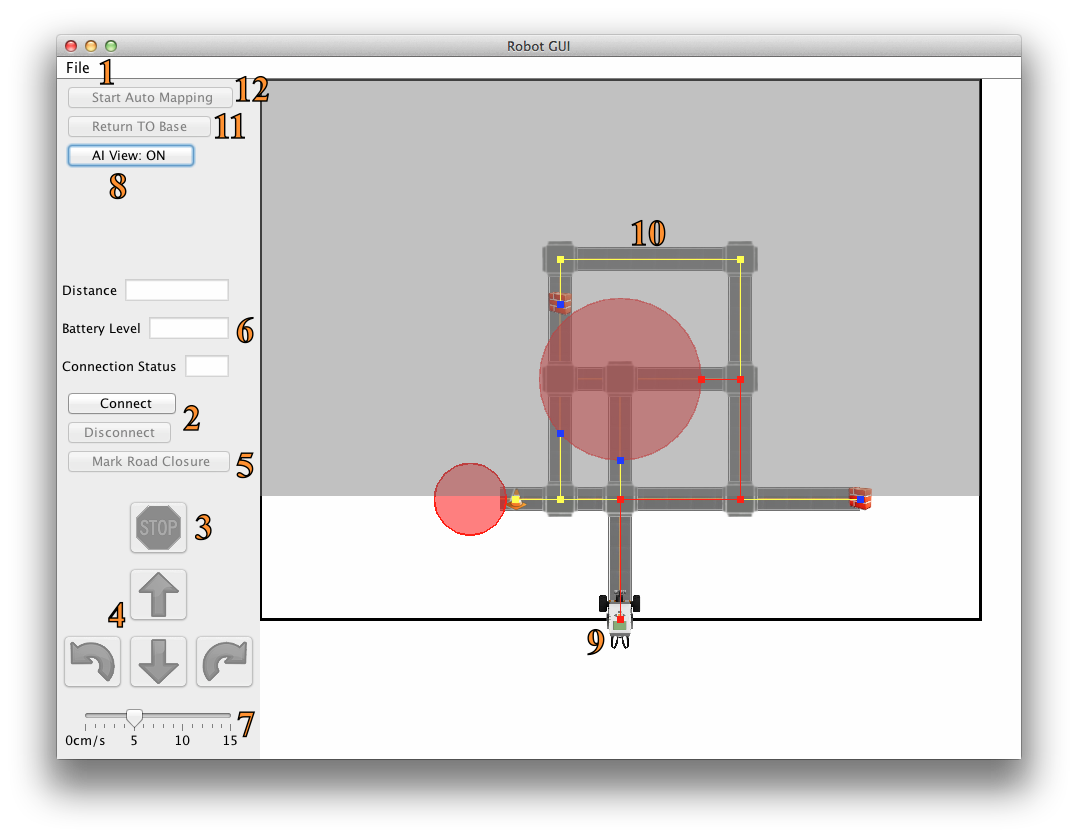
\includegraphics[scale=0.4]{GUI.png}

\subsection{[1] File Menu}
The file menu has three functions for the operator to use. The first function is "save" which allows the user to save the currently explored map to a file. The second function is "load" which allows the user to load a previously saved map. The third function of the menu is simply "quit" which closes the whole program.

\subsection{[2] Connection Buttons}
The "Connect" button is used to connect the PC to the robot. The operator may need to wait for few seconds for the PC to connect to the robot. The "Disconnect" button is used to disconnect the robot from the PC.

\subsection{[3] Emergency Stop}
The emergency "STOP" button is used when the operator needs the robot to stop immediatly. This button is useful in the situation where the robot's movement maybe dangerous to the environment around it or to the robot itself.


\subsection{[4] Manual Control Buttons}
The manual control buttons are simply used to control the robot movements when it is in the manual mode: up (forwards), down (backwards), left (rotate anti-clockwise), right (rotate clockwise). These simple functions can be also done using the arrow keys on the PC keyboard.

\subsection{[5] Mark Road Closure}
The operator can use "Mark Road Closure" button when he/she wants the robot to mark a " ) " shape road closure on the map. On the physical map, the robot will lower the pen on the paper map and move right to left to produce the mark.

\subsection{[6] Robot Information Indecators}
The indecators panel shows the ultrasonic distance, the robot's battery level and the connection status of the robot. This information display is important to keep the operator informed of the robot's status.

\subsection{[7] Robot Speed}
The operator can simply drag the slider to the right to speed up the robot movement, or slide to the left to slow down the robot movement.

\subsection{[8] AI View}
The "AI View" button is used to turn on/off AI view which shows the map components which will be mentioned in section 10.

\subsection{[9] Robot Location}
The robot shape represents the robot location. It moves and rotates as the robot moves and rotates on the map. 

\subsection{[10] Map AI Display}
The map display shows all the data points found in the explored area. it also shows road closures and obstacles and all paths which the robot followed.

\subsection{[11] Reture to Base}
The "Return TO Base" button allows the operator to make the robot go back to its starting point after exploring the map or stop the robot from exploring and return to the starting point.

\subsection{[12] Start Auto Mapping}
The "Start Auto Mpping" button is used to run the robot in the automatic mode. The robot will start to do its exploration independently without the manual guidence of the operator.

\section{Guide For Robot Control}
The following guide is an outline for basic control of the Graphical User Interface (GUI) and the robot.

\subsection{Starting the robot}
The operator needs to start the robot manually and the default program should be run. When the NXT brick LCD display shows the interface, the robot is ready to be connected to. 

\subsection{Starting the Graphical User Interface}
When the progarm is run and GUI is first loaded, most of the buttons are displayed as they are not able to be used. The two main options for the operator are connect and AI map view. It is recommended that the map is loaded before connecting to the robot but it is not necessary.

\subsection{Connecting the Robot and Loading the Map Area}
Another way to specify the map area is to load an xml file from File >  load. After pushing the connect button, the operator may need to wait for the connection to be established. Once the robot is connected The connection status bar will change to "On" indicating that the robot is finally connected.


\subsection{Starting the Manual or Automatic Survey}
The robot is now ready to start exploration. To undertake an automated mapping, click on the "Start Auto Mapping" and it will explore the area using a specified search algorithm. to stop the the search, click the stop button or the directions buttons.

\subsection{Finishing up}
When the exploration is complete, the map can be saved by clicking on File > Save. This will save the currently explored map as an xml file for later use. After this you may load a new map or simply quit the program.



\end{document}
